\documentclass[a4j,twoside,openright,11pt]{jarticle}
%
\usepackage{amsmath,amssymb}
\usepackage{bm}
\usepackage{graphicx}
\usepackage{ascmac}
\usepackage{listliketab}
\usepackage{url}
\usepackage{listings}

\setlength{\textwidth}{15.92cm}
\setlength{\oddsidemargin}{0mm}
\setlength{\evensidemargin}{0mm}
\setlength{\topmargin}{-1cm}
\setlength{\textheight}{23.5cm}
\setlength{\footskip}{18mm}

%
\pagestyle{plain}
\makeatletter
  \def\@maketitle{%
  \newpage\null
  \vskip 2em%
  \begin{center}%
  \let\footnote\thanks
    {\huge \@title \par}%
    \vskip 1.5em%
  \end{center}% 追加
  \begin{flushright}
        \@author
  \end{flushright}
  \begin{flushright}% 追加
    {\large \@date}%
  \end{flushright}%
  \par\vskip 1.5em}
\makeatother

\title{振動制御実験}
\author{九州工業大学 機械知能工学科 機械コース\\3年 学籍番号:13104069 坂本 悠作}
\date{
実験日1:平成27年6月17日\\
実験日2:平成27年6月24日\\
提出日 :平成27年6月30日
}
\begin{document}
\maketitle

\section{基本課題1}
授業内課題発表点 13
\newpage
\section{基本課題2}
\subsection{実験の感想}
機械工学実験の中では特に楽しめる内容であったと感じた。進行もスムーズに流れていたので、全体的に見れば非常に良い実験であったと感じた。
\subsection{機械・宇宙システムの技術者として、制御をどう捉えるか}
現在の機械製品では、電子機器による制御が欠かせない状態にあるため、制御の知識・技術はある程度持っておくべきことであると考える。しかし、あまりにも電子制御に頼ってしまうと現代までに培われたからくり(例えば、ゼンマイで動作する機械式時計)のような技術を継承していく者は必要であると思う。
\subsection{PID制御とはなにか}
PID制御系の最も基本的な構成は図に示す通りである。
\begin{figure}[htbp]
\begin{center}
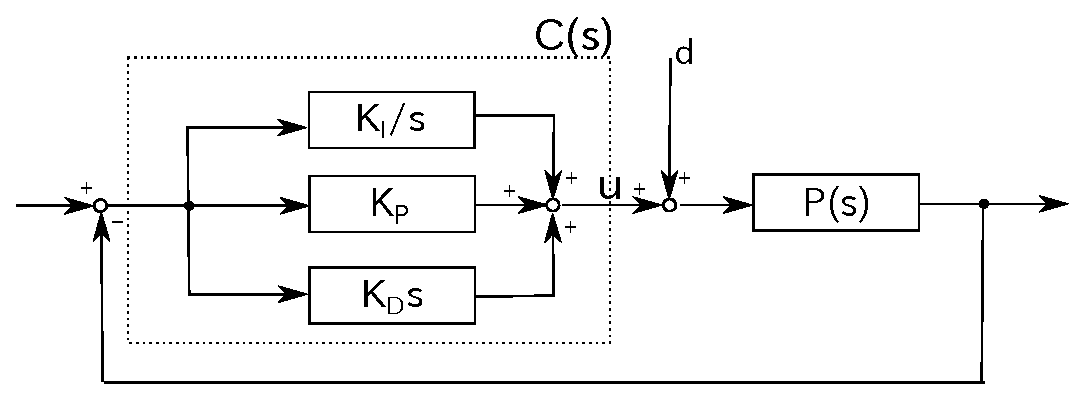
\includegraphics[width=12cm]{PID1.eps}
\end{center}
\caption{PID制御系の基本形}
\end{figure}
PID補償器$C(s)$は、比例・積分・微分の3つの要素を並列に結合したものである。$K_P,K_I,K_D$のパラメータは、それぞれ比例ゲイン・積分ゲイン・微分ゲインと呼ばれており、
\subsection{最適制御とはなにか}


\section{実験を改善する方策を述べよ}
\begin{enumerate}
\item 第1週目の倒立振子ロボットの組み立ては、目的が明確でなく時間の無駄だと感じましたのでロボットを事前に組み立てておくのがよろしいと思います。1週目2周目共に同じロボットを使用するのであれば、組み立て・分解する必要性が全く見当たりません。
\item 2周めの最適制御でのレースは必要ないと感じました。前週のPID制御でのレースとの違いが見当たらないので、もしも違いを明確に認識することが目的であったならば、違いが顕著に現れている動画等を撮影し、それを見比べる方が学習になったと思います。
\item 2周目の発表では、評価をする教員の方が完成度を求めすぎているように感じました。全員が誤解しないような言葉を使うように、という指摘ではなく、目的を絞って行なうほうがよろしいと思います。
\end{enumerate}
\section{最適制御よりもPID制御の方が非常に多くの場面で使われているのはなぜか}

\end{document}
